\section{Relative Orientation}
\label{chapter:design:coordinatesystem}

	The Cartesian \termdef{Coordinate System} of the 3-dimensional space of a scene has two properties that need to be defined in order to position objects therein:

	\begin{smalllist}
		\item Handedness: The direction the third vector points to, when the first two are defined.
		\item Orientation: The directions the three vectors point to relative to the render window.
	\end{smalllist}

	The orientation is unnecessary for the definition of the coordinate system from a mathematical point of view, since all orientations with the same handedness can be transformed to each other using a single rotation around the origin according to Euler's rotation theorem\cite{PP07}. But since human orientation rather happens in terms of relative directions -- up, down, left, right, forward, backward -- we will try to use these directions instead of the named axes $X$, $Y$ and $Z$.

	The lack of a standard mapping\footnote{OpenGL and Direct3D9 both use X/Y for left/up but differ in handedness, OpenGL defining negative Z as the forward vector\cite{Buss:2003:CGM:861813}, whereas Direct3D9 chooses positive Z\cite{jones2004beginning}. Panda3d, on the other hand, implements a right-handed coordinate system where X, Y and Z correspond to right, forward and upward\cite{Goslin:2004:PGE:1032275.1032359}.} is taken as an indicator that it is best left to personal preference. The choice will not have any effect on the API if orientation is expressed throughout the application, but it will still have two effects on the result:

	\begin{smalllist}
		\item If relative movement using the terms ``up'' or ``down'' are used alongside vectors for positioning objects, the three components of the vector will each map to one relative direction. There will be a visible difference between the exact same applications using different coordinate systems.
		\item The other implication is not so obvious: The underlying renderer will need to perform additional operations if the handedness of the coordinate systems differs from its own usage. We will elaborate on this effect during the implementation of the \classname{Renderer} in Section \ref{chapter:implementation:renderer}.
	\end{smalllist}

	Conceptually, the desired orientation serves but a single purpose: to assign a default rotation to newly created objects. All rotatable objects have a predefined orientation, or predefined directions that are considered that object's forward, right and up vectors. The orientation of the coordinate system rotates all new objects to align those directional vectors to those of the coordinate system's orientation. Figure \ref{fig:RotatedSpotLight} shows a newly created spot light that was positioned facing forward in the coordinate system orientation of Direct3D9 -- assuming that the forward orientation of a spot light is defined by the direction vector its light is emitted to.

	As long as the coordinate system to use during development is defined before any objects have been created, the library does not need to care about the coordinate system in use. We will need to define how the application behaves if the coordinate system is changed at run-time:

	Although it would technically be possible to re-position all objects within the scene, we have chosen to ignore this event. Although changing the coordinate system after having used it for positioning can lead to unexpected results, it is still possible to set the desired coordinate system at any point during run-time. The responsibility for choosing a system before starting the scene setup is left to the developer.
	
	Since changing the coordinate system of a project during development would lead to quite unexpected behavior, this constraint appears acceptable. We will be using the OpenGL standard as the default coordinate system in our library if no other system is set explicitly.

	\begin{figure}[htbp]
		\centering
		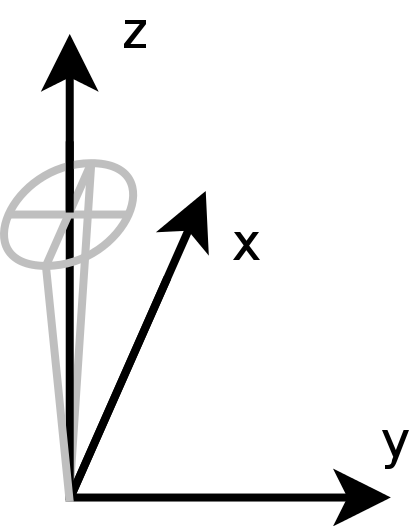
\includegraphics[width=4cm]{images/rotatedspotlight.png}
		\caption{A spot light facing ``forward'' in the Direct3D9 coordinate system, assuming its front-side is the direction the light is emitted to.}
		\label{fig:RotatedSpotLight}
	\end{figure}

	Although such relative axes are defined in all graphics engines, they are not an integral part of the API. The orientation serves a more technical purpose: When the scene is viewed from a certain point, every other object is positioned in a coordinate system that has its origin at that point. All objects left of the viewer have a negative $X$ value in OpenGL or Direct3D9 at this point. The mapping of named axes to the relative directions are only performed, as the whole scene is transformed into this coordinate system eventually.

	The orientation is still used as a default alignment of new objects but a ``rotation to the left'' does not exist in any of the reference APIs\footnote{Although Ogre3d provides equivalent methods called \inlinecode{yaw()}, \inlinecode{pitch()} and \inlinecode{roll()}, the wording is intentionally chosen \emph{not} to resemble orientation relative to the current position.}, rendering the original definition less useful than it could be. Whatever the orientation of the coordinate system is, one must fall back to the usage of the named coordinate axes $X$, $Y$ and $Z$ during application development.

	We will introduce relative orientation into the API to make stronger use of the already-present orientation capabilities of humans in the real world. If the Direct3D9 alignment of the coordinate system was chosen, a rotation around the $Y$ axis can be expressed as a rotation to the right: \inlinecode{rotateRight(Degree(90));}.

	A problem with an approach using this model is the ambiguity of the reference position. A very good example one is immediately confronted with when getting acquainted with a graphics library API is the rotation of a camera. We will start to explore this issue by defining three distinct axes along which one could perform rotations in our relative coordinate system. These axes reach
	
	\begin{smalllist}
		\item from left to right,
		\item from down to up and
		\item from backward to forward.
	\end{smalllist}

	The problem with cameras is that the human brain is not used to process tilted images. A camera that was rotated along the backward-forward axis tends to look odd, as demonstrated by Figure \ref{fig:TiltedCamera}. This means that the rotational axes for the default use of cameras can be reduced to two:
	
	\begin{figure}[htbp]
		\centering
		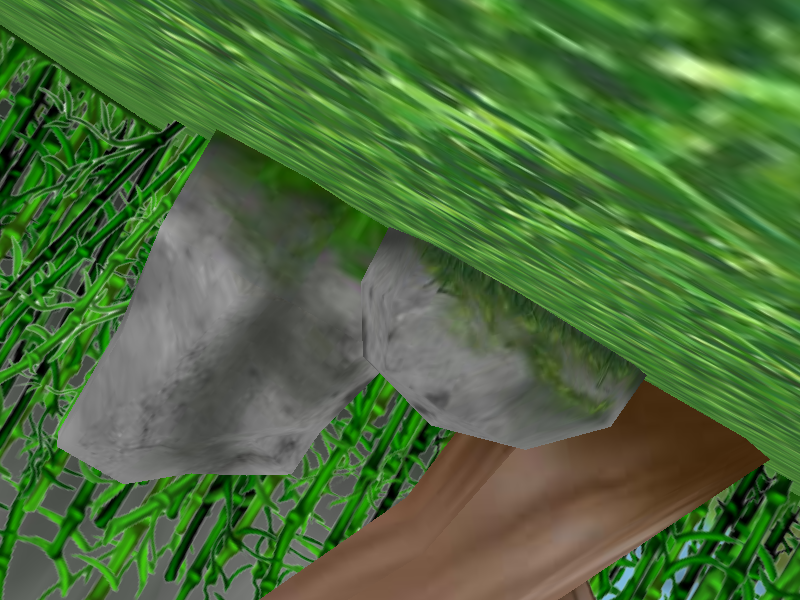
\includegraphics[width=14cm]{images/tiltedcamera/cam.png}
		\caption{A tilted camera}
		\label{fig:TiltedCamera}
	\end{figure}

	\begin{smalllist}
		\item from left to right (for looking up/down) and
		\item down to up (for looking to the sides).
	\end{smalllist}

	The next issue arises when these two axes are used consecutively. A camera that was rotated to look downward -- a rotation along the left-right axis -- a rotation along the down-up axis -- with the intention of looking sideways -- introduces an amount of tilt. This phenomenon is a result of the rotation along a local axis -- the tilt of the object has not changed from the viewpoint of the camera object itself, but the tilt of the current orientation of the camera has -- from the viewpoint of an unrotated scene node, as seen in Figure \ref{fig:CameraRotation}.

	\begin{figure}[htbp]
		\centering
		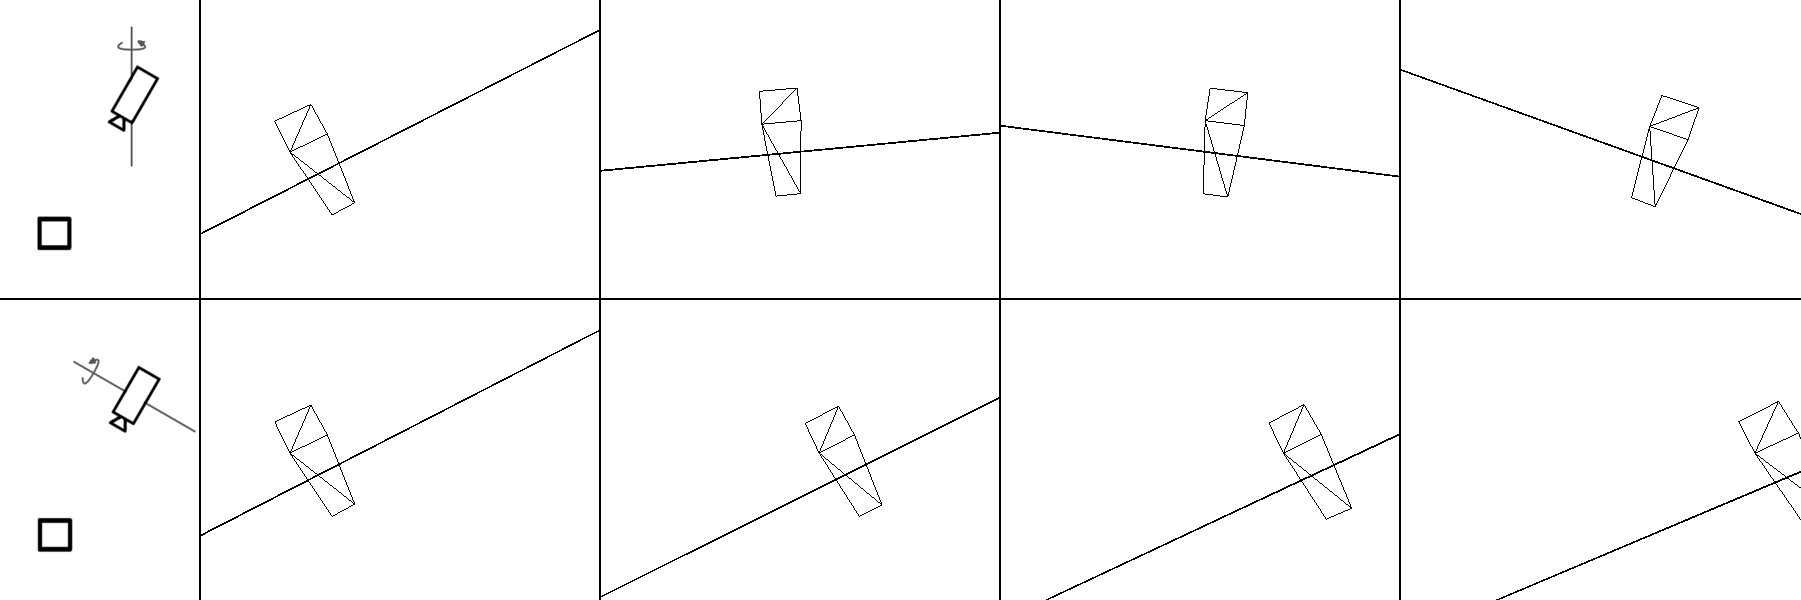
\includegraphics[width=14cm]{images/camera/camera.png}
		\caption{Rotating a camera looking down on a cube around the global coordinate system (upper frames) and its local coordinate system (lower frames). The lower images demonstrate that the tilt of the camera has not changed within its local coordinate system: the line on the floor is always parallel to that in other frames.}
		\label{fig:CameraRotation}
	\end{figure}

	The available rotation axes to a camera are further constrained to

	\begin{smalllist}
		\item the \emph{local} axis traversing from left to right and
		\item the \emph{global} axis pointing upwards.
	\end{smalllist}

	This example demonstrates the main issue with rotations. Every rotation consists of two distinct components:

	\begin{numlist}
		\item an axis/angle pair that defines the rotation and
		\item the coordinate system the rotation is to be performed in.
	\end{numlist}

	There are two approaches in our reference engines to the ambiguity arising due to the non-commutative nature of quaternion multiplication during rotations. Prior to these solutions, we must take note that all reference engines use quaternions for the orientation within the scene. The following is an example in Ogre3d:

	% leading whitespace in the following code snippet must consist of spaces, not tabs!
	\begin{code}[2]
		Quaternion rotation1;
		Quaternion rotation2;
		rotation1.FromAngleAxis(Degree(90), Vector3::UNIT_Y)
		rotation2.FromAngleAxis(Degree(90), Vector3::UNIT_X)
		sceneNode->rotate(rotation1 * rotation2);
	\end{code}

	The quaternions are used differently by our reference engines, though:

	\begin{smalllist}
		\item Ogre3d's \classname{SceneNode} has a method \inlinecode{rotate()} that accepts a quaternion as first, and the \classname{TransformSpace} as second parameter. The \classname{TransformSpace} is an enum consisting of the values
		\begin{smalllist}
			\item \inlinecode{TS\_LOCAL} -- rotation within the current orientation, this is the default value of this parameter
			\item \inlinecode{TS\_PARENT} -- rotation within the orientation of the parent scene node
			\item \inlinecode{TS\_WORLD} -- rotation from the viewpoint of an unrotated scene node
		\end{smalllist}
		\item The other libraries do not provide any means of rotating rotated nodes at all. The only option is to \emph{re-set} the orientation of a scene node. The developer is responsible for the creation of the desired quaternion for this purpose.
	\end{smalllist}

	Although Ogre3d uses three predefined context spaces, the rotation is not limited to those three, so we will approach the issue from a different angle. Instead of limiting the contexts to these values, we will declare that a rotation requires a \emph{context node} the operation is performed in. In the camera example above, this is either the parent node (casually referred to as ``local'' value above), or the root node of the scene graph (the ``global'' value).

	Every node should actually be viewed as a coordinate system that is embedded into another coordinate system\footnote{Except for the root node, which does not have a parent}. In other words: every child node creates a sub-space within its parent node. This means that the global result of a rotation will change depending on the space the query is performed in.

	%\begin{minipage}{15.35cm}
	\begin{code}[2]
		sceneNode->rotate(quaternion, context);
	\end{code}
	%\end{minipage}

	This choice brings up an ambiguity: it is not clear, whether the \inlinecode{context} implies an \emph{orientation} or a \emph{location}. The above code snippet could be interpreted as either of:

	\begin{smalllist}
		\item ``Perform the rotation as if the \inlinecode{context} node was looking at \inlinecode{sceneNode} from its current \emph{position}.''
		\item ``Perform the rotation as if the \inlinecode{context} node was re-positioned to look at \inlinecode{sceneNode} without changing its \emph{orientation}.''
	\end{smalllist}

	We have accepted this flaw and kept this solution, since the behavior during re-orientation is application-specific -- a camera would probably be rotated differently than an asteroid floating in space without gravity. Re-positioning a node leaves much less room for interpretation: the only remaining variable is the distance to the object, which is irrelevant for this purpose.

	The implementation of the concepts described here can be found in Section \ref{chapter:implementation:scenegraph}.

